%
% ****
\chapter{Implementierung des TW-Netzes}
\label{chap:imp}
% ****
%

	\begin{minipage}[b]{0.65\textwidth}
		Die Implementierung des gesamten neuronalen Netzes inklusive der Simulationsumgebung erfolgt in der Programmiersprache \texttt{Python}. Als Module werden zum einen das bereits vorgestellte Leaky Integrate and Fire - Modell implementiert, zum anderen diverse Algorithmen zur Suche von individuellen Parametern des neuronalen Netzes. Darüber hinaus ist das Programm in der Lage, eine Simulation der gefundenen Parameter durch die Simulationsumgebung \texttt{CartPole\_v0} von OpenAI Gym zu zeigen und Parameter über die Simulationszeit zu plotten. Die Module sowie diverse Dokumentationen und Informationen sind in meinem GitHub-Repository\footnotemark{} zu finden. Ein entsprechendes Deckblatt mit weiteren Informationen liegt dieser Arbeit in Anhang \ref{app:parameter} bei.
	\end{minipage}
	\begin{minipage}[b]{0.35\textwidth}
		\begin{figure}[H] %[!t] ...
			\centering
			
\includegraphics[width=5cm]{figures/appendix/qr-code.pdf}
			\caption{QR-Code Verweis zum GitHub-Repository.}
			\label{fig:qr}
		\end{figure}
	\end{minipage}
	\footnotetext{https://github.com/J0nasW/BA}
		

% ***
\section{Aufbau des Programms}
\label{sec:imp_module}
% ***
	Ein Ziel dieser Arbeit ist es, neben der Funktionstüchtigkeit des Simulators das entstandene Programm mitsamt allen Modulen und Abhängigkeiten modular und leicht verständlich aufzubauen. Dazu gehört eine gute Dokumentation sowie saubere Versionierung, um Änderungen nachvollziehbar darzustellen.\\
	Folgende Anforderungen werden an das Programm gestellt:
	\begin{itemize}
		\item Es existiert ein zentraler Punkt zum Ändern aller nötigen Parameter. Alle weiteren Größen werden durch Formeln und Abfragen erzeugt.
		\subitem Datei: \texttt{parameters.py}
		\item Es wird ein Modul zur Visualisierung gegebener Parameter oder Gewichte des neuronalen Netzes bereitgestellt. Diese Datei muss leicht verständlich und manipulierbar sein, um eigene Plots zu erstellen und neue Simulationsumgebungen einzubinden.
		\subitem Datei: \texttt{visiualize.py}
		\item Es muss die Möglichkeit bestehen, aus bereits existierenden Suchalgorithmen neue Implementationen zu erstellen und gegebene Funktionen einfach einsetzen zu können.
		\subitem Vorlage: \texttt{random\_search\_v2.py}, \texttt{weights\_nn.py}
	\end{itemize}
	Aufgrund der hohen Vielfältigkeit an neuronalen Netzen und Suchalgorithmen soll dieses Programm als Basis für neue Projekte und Ideen dienen. Daher wird empfohlen, eine Fork des Repositories (siehe Anhang \ref{app:parameter}) zu erstellen und den Simulator weiter zu gestalten.\\
	Das Programm beinhaltet folgende Module:\\
	\begin{minipage}{0.35\textwidth}
		\vspace{0.3cm}
		\begin{forest}
			pic dir tree,
			where level=0{}{% folder icons by default; override using file for file icons
				directory,
			},
			[TW Circuit
				[docs]
				[information]
				[modules
					[inspect.py, file]
					[lif.py, file]
					[parameters.py, file]
					[random\_search\_v2.py, file]
					[visiualize.py, file]
					[weights.py, file]]
				[parameter\_dumps]
				[weight\_dumps]
				[main.py, file]]
		\end{forest}
	\end{minipage}
	\begin{minipage}{0.65\textwidth}
		\begin{itemize}
			\item Der Ordner \texttt{docs} beinhaltet wichtige Dokumentationen bezüglich des Codes und dem Umgang mit diversen Befehlen innerhalb der \texttt{main.py}. Darüber hinaus wird hier ebenfalls diese Arbeit inklusive des \LaTeX-Codes abgelegt.
			\item Aufgrund vieler komplexer Simulationen mit verschiedenen Parametersätzen wurde die Berechnung von Heim- und Unirechnern auf Rechenzentren ausgelagert. Der Ordner \texttt{information} wird genutzt, um Informationen über jede Simulation (Ergebnisse, Zeitstempel, Zugehörigkeit, ...) in Form einer TXT-Datei zu speichern.
			\item Alle nötigen Module zur Simulation und Visualisierung finden sich in dem Ordner \texttt{modules} wieder. Genauere Informationen zu den einzelnen Skripten werden in den nächsten Sektionen aufgeführt.
			\item parameter\_dumps und weight\_dumps sind die Resultate der Simulationsläufe. In diesen Ordnern werden Parameter und Gewichte des neuronalen Netzes nach erfolgreichen Simulationsläufen abgespeichert. Die Dateien werden durch das Skript \texttt{hickle} in ein HDF-5 Dateiformat \cite{hdf5} gespeichert.
		\end{itemize}		
	\end{minipage}
	
	
		
% ***
\section{Implementierung der Suchalgorithmen}
\label{sec:imp_search}
% ***
	Die Suchalgorithmen befinden sich jeweils in dem Ordner \texttt{modules} und werden durch Import in der Datei \texttt{main.py} aufgerufen. Sie erhalten bei Aufruf die vom Anwender gewählte Simulationszeit (bspw. 12 Stunden) und bei Bedarf bereits errechnete Parameter. Als Ausgabe wird ein Dump der errechneten Parameter oder Gewichte gespeichert sowie eine Informationsdatei, welche Zugehörigkeiten, Anz. an Simulationen, Laufzeiten und den gesamten Reward beschreibt. 
	
	\subsection{Suchalgorithmus RandomSearch}
		Der Suchalgorithmus RandomSearch wurde direkt in die Simulation eingebunden. Es werden die Parameter $C_m, G_{Leak}, U_{Leak}, \sigma, w, \hat{w}$ durch eine Gleichverteilung in den bereits genannten Grenzen zufällig erzeugt. Um gleich-verteilte, zufällige Werte zu generieren, wird die Funktion \texttt{random.uniform} aus dem bekannten Package \texttt{numpy} \cite{NumPy} verwendet.
		\begin{algorithm}
			\SetKwInOut{Input}{Input}
			\SetKwInOut{Output}{Output}
			
			\Input{Anz. Nervenzellen, Anz. Synapsen, Anz. Gap-Junctions}
			\Output{Arrays $\boldsymbol{C_m, G_{Leak}, U_{Leak}, \sigma, w, \hat{w}}$}
				\tcp{Generieren von Zufallsvariablen durch Gleichverteilung.}
				\tcp{Für Nervenzellen:}
				$\boldsymbol{C_m}$ = np.random.uniform(low = 0.01, high = 1, size = (1,Anz. Nervenzellen))\\
				$\boldsymbol{G_{leak}}$ = np.random.uniform(low = 0.05, high = 5, size = (1,Anz. Nervenzellen))\\
				$\boldsymbol{U_{leak}}$ = np.random.uniform(low = -70, high = 0, size = (1,Anz. Nervenzellen))\\
				\tcp{Für Synapsen:}
				$\boldsymbol{\sigma}$ = np.random.uniform(low = 0.05, high = 0.5, size = (1,Anz. Synapsen))\\
				$\boldsymbol{w}$ = np.random.uniform(low = 0, high = 3, size = (1,Anz. Synapsen))\\
				$\boldsymbol{\hat{w}}$ = np.random.uniform(low = 0, high = 03, size = (1,Anz. Gap-Junctions))
				\KwRet{$\boldsymbol{C_m, G_{Leak}, U_{Leak}, \sigma, w, \hat{w}}$}	
			\caption{random\_parameters}
		\end{algorithm}
		Nach Aufruf des Algorithmus \texttt{random\_parameters} wird eine Simulation mit den erzeugten Parametern und maximal 200 Zeitschritten durchgeführt. Der Reward dieser Simulation wird mit vergangenen Rewards verglichen. Wenn die Simulation einen Reward größer oder gleich 200 erreicht, gilt sie erfolgreich, andernfalls wird nach Ablauf der Simulationszeit der Algorithmus unterbrochen.\\
		Der gesamte Programmablauf gestaltet sich vereinfacht wie folgt:
		\begin{algorithm}
			\SetKwInOut{Input}{Input}
			\SetKwInOut{Output}{Output}
			
			\Input{Simulationszeit}
			\Output{Simulationsinformation (information.txt), Parameter-Dump als .hkl Datei}
			
			action = episodes = best\_reward = 0\\
			env = gym.make('CartPole-v0')\\
			\While{True}{
				initialize(Default\_U\_leak)\\
				episodes $\leftarrow$ episodes + 1\\
				$\boldsymbol{C_m, G_{Leak}, U_{Leak}, \sigma, w, \hat{w}}$ = random\_parameters()\\
				reward = run\_episode($\boldsymbol{C_m, G_{Leak}, U_{Leak}, \sigma, w, \hat{w}}$) \tcp*{Simulation mit neuen Parametern - Siehe Sec. \ref{sec:imp_sim}}
				\If{reward $\geq$ best\_reward}{
					Set best\_reward $\leftarrow$ reward\\
					Result = [$\boldsymbol{C_m, G_{Leak}, U_{Leak}, \sigma, w, \hat{w}}$] \tcp*{Für Parameter-Dump}
					\If{reward $\geq$ 200}{
						\textbf{break}\tcp*{Exit-Argument, wenn Reward von 200 erreicht wurde}
					}
				}
				\If{elapsed\_time $>$ simulation\_time}{
					\textbf{break} \tcp*{Exit-Argument, um genaue Laufzeiten zu erzielen}
				}
			}
			\KwRet{information.txt, parameter\_dump.hkl, date, best\_reward}
			\caption{random\_search\_v2}
		\end{algorithm}\\
		Die elementare Funktion \texttt{run\_episode} wird in Sektion \ref{sec:imp_sim} genauer erläutert. Sie enthält unter anderem auch die Funktion \texttt{compute}, welche in Sektion \ref{sec:lif_imp} bereits detailliert thematisiert wurde.
	\subsection{Optimierungsalgorithmus Weights}
		Als erstes Optimierungsverfahren nach erfolgreicher Simulation der Parameter des neuronalen Netzes wird nun der Algorithmus Weights eingesetzt. Dieser lässt die bereits simulierten Parameter importieren und gewichtet jede Synapse mit einem Faktor $g\in[0,1]$. Durch einfache Simulationen mit willkürlichen Gewichten wird schnell festgestellt, welche Synapsen bei einem Simulationslauf mit hohem Reward eine große Gewichtung erhalten und welche Synapsen nicht förderlich für das Ergebnis sind. Durch diese Simulation war es möglich, das in Kap. \ref{chap:neuro} vorgestellte symmetrische Neuronale Netz (Abb. \ref{fig:nn_new}) zu entwickeln. Die dort gezeigten Synapsen erfahren eine relevante Gewichtung und sind somit wichtig für den Erfolg des neuronalen Netzes.\\
		Der Gewichtungsalgorithmus ist rechenintensiver als RandomSearch, da insgesamt 16 Synapsen bzw. Gap-Junctions pro Episode mit zufällig gewählten Gewichten versehen werden, um den Reward zu steigern. Jedoch wird ein im Schnitt um das Dreifache höherer Reward verzeichnet bei gleichbleibenden Parametern, was eine sehr gute Optimierung darstellt.\\
		Aufgerufen wird dieser Algorithmus analog zu RandomSearch aus der \texttt{main.py}-Datei. Als Input werden die bereits errechneten optimalen Parameter der jeweiligen Nervenzellen und Synapsen sowie die maximale Simulationszeit eingegeben. Ebenfalls gleich dem Algorithmus RandomSearch produziert Weights einen Dump mit den errechneten Gewichten der Synapsen und Gap-Junctions sowie eine Informationsdatei im \texttt{.txt}-Format, welche weitere Zugehörigkeitsinformationen sowie die Anzahl an Simulationen und die Dauer enthält.
		
	\subsection{Simulation in der Google Cloud Platform\textsuperscript{\textregistered}}
		Wie bereits in diesem Abschnitt mehrfach erwähnt, sind die implementierten Suchalgorithmen RandomSearch und Weights äußerst rechenintensiv. Beide Skripte erfordern das zufällige Generieren einer hohen Anzahl an Parametern sowie die Anwendung dieser Parameter auf das gegebene Problem durch numerische Lösungsansätze für Differenzialgleichungen (siehe Sektion \ref{sec:lif_imp}). Es müssen Parameter zwischengespeichert und Dumps auf Festplatten geschrieben werden.\\
		Um eine erfolgreiche Simulation des inversen Pendels zu erhalten, muss ein Parametersatz mit hohem Reward gefunden werden, welcher die korrekte Funktionsweise des neuronalen Netzes gewährleistet. Bei dem in Abb. \ref{fig:nn_new} gezeigten neuronalen Netz werden die Parameter $C_m, G_{Leak}, U_{Leak}, \sigma, w, \hat{w}$ für Synapsen, Gap-Junctions und Nervenzellen simuliert.
		\begin{center}
			\begin{tabular}{c@{\hskip 0.5cm}c@{\hskip 0.5cm}c@{\hskip 0.5cm}}    \toprule
				\setlength{\tabcolsep}{50pt}
				\renewcommand{\arraystretch}{1.5}
				\emph{Parameter}	& \emph{Kategorie}  & \emph{Anzahl} \\\midrule
				$C_m$				& Nervenzelle		& 4				\\ 
				$G_{Leak}$	 		& Nervenzelle		& 4				\\
				$U_{Leak}$	 		& Nervenzelle		& 4				\\
				$\sigma$			& Synapse			& 16			\\
				$w$					& Synapse			& 16			\\ 
				$\hat{w}$			& Synapse			& 2				\\\bottomrule
				Gesamt:				&					& \textbf{46}	\\
				\hline
			\end{tabular}
		\end{center}
		Somit werden in jedem Simulationslauf zuerst 46 Parameter in gegebenen Grenzen durch eine Gleichverteilung erzeugt und anschließend durch das \texttt{compute}-Modul (siehe Sektion\ref{sec:lif_imp}) die benötigten Synapsenströme und Membranpotentiale errechnet.\\
		Das Modul Weights erzeugt, analog zu RandomSearch, zuerst für jede Synapse und Gap-Junction ein gleich-verteiltes, zufälliges Gewicht $g\in[0,1]$.
		\begin{center}
			\begin{tabular}{c@{\hskip 0.5cm}c@{\hskip 0.5cm}c@{\hskip 0.5cm}}    \toprule
				\setlength{\tabcolsep}{50pt}
				\renewcommand{\arraystretch}{1.5}
				\emph{Parameter}	& \emph{Kategorie}  & \emph{Anzahl} \\\midrule
				$g$					& Synapse			& 18			\\\bottomrule
				Gesamt:				&					& \textbf{18}	\\
				\hline
			\end{tabular}
		\end{center}
		Somit werden insgesamt 18 Gewichte pro Episode erzeugt und auf das Modell angewendet. Zur Berechnung der erforderlichen Ströme und Potenziale wird das \texttt{compute}-Modul um die Funktion der Gewichtung erweitert.\\
		Ein solches Simulationsvorhaben wird üblicherweise nicht mehr auf Heimrechnern ausgeführt, sondern findet den Weg in die Cloud. Gerade in den letzten Jahren haben Cloud-Computing-Firmen wie Amazon mit AWS\footnote{https://aws.amazon.com/de/}, Microsoft mit der Azure Cloud\footnote{https://azure.microsoft.com/de-de/} und Google mit der Google Cloud Platform (GCP)\footnote{https://cloud.google.com/} an großer Aufmerksamkeit gewonnen. Die einfache Handhabung und Kontrolle über eigene virtuelle Instanzen von ganzen Betriebssystemen erlaubt eine zuverlässige und effiziente Simulation von Parametern. In dieser Angelegenheit wurde sich für die Google Cloud Plattform entschieden, da diese ein sehr gutes User Inferface hat und kostengünstige, virtuelle Maschinen anbietet. Gemietet wurde ein Server mit dem Standort Frankfurt, welcher über vier virtuelle Intel XEON\textsuperscript{\textregistered} Prozessoren sowie 12GB DDR4 Arbeitsspeicher verfügt. Dies erlaubt eine schnelle Simulation von vier Instanzen zur gleichen Zeit sowie den Vorteil, das Langzeitsimulationen von 12 Stunden oder mehr im Hintergrund oder über Nacht erfolgen können.\\
		Auf der virtuellen Instanz wurde ein Linux Ubuntu 18.04 LTS installiert und bereitgestellt. Im nächsten Schritt wird die vorbereitete GitHub Repository auf das System geklont und die benötigten Abhängigkeiten (siehe Anhang \ref{app:datenblatt}) installiert. Durch einen Cronjob werden Skripte ausgeführt und mit \texttt{crontab -e} die Simulation zu einer festen Uhrzeit gestartet. Die übliche Simulationszeit beträgt jeweils 12 Stunden.\\
		\begin{minipage}[c]{0.5\textwidth}
			\begin{figure}[H] %[!t] ...
				\centering
				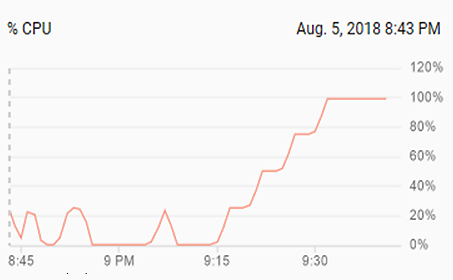
\includegraphics[width=7cm]{figures/chap_implement/GCP.png}
				\caption{Systemauslastung der virtuellen Instanz - GCP Dashboard}
				\label{fig:gcp_1}
			\end{figure}
		\end{minipage}
		\begin{minipage}[c]{0.5\textwidth}
			\begin{figure}[H] %[!t] ...
				\centering
				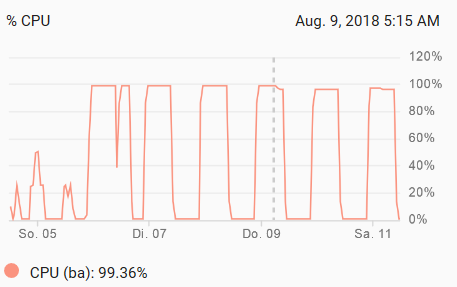
\includegraphics[width=7cm]{figures/chap_implement/GCP_2.png}
				\caption{Systemauslastung der virtuellen Instanz im Dauerbetrieb (Cronjob)}
				\label{fig:gcp_2}
			\end{figure}
		\end{minipage}\vspace{0.5cm}
		Wie in Abb. \ref{fig:gcp_1} und \ref{fig:gcp_2} zu sehen, werden die Suchalgorithmen nacheinander durch den Cronjob ausgeführt, da pro Suchlauf nur ein Prozessorkern in Anspruch genommen werden kann. Der virtuelle Prozessor erreicht somit bei vier gleichzeitigen Simulationsläufen eine Auslastung von $100\%$.\\
		Die Ergebnisse der Suchläufe werden in Form von Parameter- und Weight-Dumps via eines Apache Webservers bereitgestellt und können problemlos auf dem Heimrechner visualisiert werden. Durch das gewählte Dateiformat der Dumps in HDF5 \cite{hdf5} sind die Dateien Plattformunabhängig und äußerst performant lesbar. Diese Methode funktioniert darüber hinaus auch Versionsübergreifend. Eine Simulation kann Dumps mit Python 2.7 erstellen, welche durch einen Heimrechner mit Python 3.x visualisiert werden können.

% ***
\section{Simulationsumgebung: OpenAI Gym}
\label{sec:imp_sim}
% ***
	Um die Performance eigener neuronaler Netze und Algorithmen zu messen, wurden in den letzten Jahren eine ganze Reihe an Simulationen und Spielen entwickelt. Ziel dieser Simulationsumgebungen ist es, die Entscheidung des Agenten in gewissen Situationen zu testen und den Lernerfolg darzustellen. Darüber hinaus wird das Verständnis für neuronale Netze durch das Anwenden auf Spiele und Experimente vertieft.\\
	Eine sehr bekannte Open Source Bibliothek an Simulatoren und Spielen ist Gym von OpenAI\footnote{https://openai.com/}. OpenAI ist eine Non-Profit Organisation mit dem Ziel, den Forschungsbereich der künstlichen Intelligenz voran zu treiben und ein besseres Verständnis für die Vorgänge in neuronalen Netzen zu schaffen. Die Bibliothek Gym enthält verschiedene Umgebungen:
	\begin{itemize}
		\item Algorithmen:
		\subitem Einfache Aktionen wie Copy-Paste, Addition und Subtraktion sowie logische Gatter
		\item Atari
		\subitem Sammlung an klassischen Atari Spielen wie Breakout, Pacman und Space Invaders
		\item Classic Control
		\subitem Simulationsumgebungen wie das inverse Pendel oder das Mountain Car
		\item Robotics
		\subitem Komplexe Simulationen von Roboterarmen oder -händen
	\end{itemize}
	In dieser Arbeit wird die Umgebung \texttt{CartPole\_v0} (Abb. \ref{fig:imp_cartpole}) gewählt. Diese besteht aus einem einfachen inversen Pendel, welches sich auf einer zweidimensionalen Bahn frei bewegen kann.
	\begin{figure}[H] %[!t] ...
		\centering
		\def\svgwidth{12cm}
		\input{figures/chap_implement/cartpole.pdf_tex}
		\caption{Simulationsumgebung \texttt{CartPole\_v0}.}
		\label{fig:imp_cartpole}
	\end{figure}
	Die Handhabung dieser Simulationsumgebung ist dank einer großen Community und guten Dokumentationen sehr einfach. Initialisiert wird die Umgebung, indem die Bibliothek \texttt{gym} in das Python-Skript importiert und die gewählte Umgebung als \glqq Environment\grqq{}festgelegt wird. Pro Simulationsschritt kann eine Aktion $a = \{0,1\}$ getätigt werden.
	\begin{align*}
		0 :& \text{ Schritt nach Links}\\
		1 :& \text{ Schritt nach Rechts}
	\end{align*}
	Das bereits vorgestellte neuronale Netz (Abb: \ref{fig:nn_new}) verfügt über zwei Motor-Neuronen, welche als Eingang der Simulation genutzt werden können. Interne Nervenzellen \textit{AVA} und \textit{AVB} sind durch eine direkte Synapse mit den genannten Motor-Neuronen verbunden und verursachen im Falle eines Fire-Events die Bewegung des Wagens um einen Schritt nach links bzw. rechts. Pro Simulationsschritt erfolgt je nach Observation immer ein Fire-Event, sodass das Pendel zu jeder Zeit eine berechnete Aktion erhält.
	\begin{figure}[H] %[!t] ...
		\centering
		\def\svgwidth{12cm}
		\input{figures/chap_implement/cartpole_FWD_REV.pdf_tex}
		\caption{Simulationsumgebung \texttt{CartPole\_v0} mit Aktionen \textit{FWD} und \textit{REV}.}
		\label{fig:imp_cartpole_FWD_REV}
	\end{figure}
	Pro Simulationsschritt wird ein Observationsvektor ausgegeben. Dieser enthält die folgenden Parameter:
	\begin{align}
		\boldsymbol{o} &= \begin{pmatrix}C_{Position} & C_{Velocity} & P_{Angle} & P_{Velocity}\end{pmatrix}\text{.}
	\end{align}
	\begin{center}
		\begin{tabular}{c@{\hskip 0.5cm}c@{\hskip 0.5cm}r@{\hskip 0.5cm}}    \toprule
			\setlength{\tabcolsep}{50pt}
			\renewcommand{\arraystretch}{1.5}
			\emph{Parameter}	& \emph{Beschreibung}  				& \emph{Grenzen} 			\\\midrule
			$C_{Position}$		& Position des Carts				& $[-2.4, 2.4]$				\\
			$C_{Velocity}$		& Geschwindigkeit des Carts			& $(-\infty, \infty)$		\\
			$P_{Angle}$			& Winkel des Pendels				& $[-41,8^{\circ}, 41,8^{\circ}]$	\\
			$P_{Velocity}$		& Winkelgeschwindigkeit des Pendels	& $(-\infty, \infty)$		\\\bottomrule
			\hline
		\end{tabular}
	\end{center}
	\begin{figure}[!h] %[!t] ...
		\centering
		\def\svgwidth{12cm}
		\input{figures/chap_implement/cartpole_observation.pdf_tex}
		\caption{Simulationsumgebung \texttt{CartPole\_v0} mit Observationsgrößen.}
		\label{fig:imp_cartpole_observation}
	\end{figure}
	Die Informationen aus dem Observationsvektor $\boldsymbol{o}$ werden entsprechend interpretiert und den Sensor-Neuronen zugeführt. Wie bereits in Sektion \ref{sec:neuro_netz} beschrieben, ist der Winkel des Pendels $\varphi$ als primäre Größe den Sensor-Neuronen \textit{PLM} und \textit{AVM} zuzuführen. Als sekundäre Größe kann die Winkelgeschwindigkeit $\dot{\varphi}$ oder die Position des Carts $x$ den Sensor-Neuronen \textit{ALM} und \textit{PVD} zugeführt werden. Die Wahl der geeigneten sekundären Observationsgröße ist dem neuronalen Netz zuzuschreiben. Durch die inhibitorische Beeinflussung durch Sensor-Neuronen \textit{ALM} und \textit{PVD} entsteht ein dämpfendes Signal, welches dafür sorgt, dass bei zu hoher Winkelgeschwindigkeit oder Cartposition die Kompensation durch Bewegung des Carts nicht übersteuert. Ergebnisse durch Wahl der geeigneten sekundären Sensorgröße werden in Kapitel \ref{chap:erg} erläutert.

% ***
\section{Visualisierung und Auswertung}
\label{sec:imp_vis}
% ***
	Wie bereits in Sektion \ref{sec:imp_sim} näher beschrieben, liefert die Simulationsumgebung \texttt{CartPole\_v0} eine sehr gute Echtzeitvisualisierung des inversen Pendels als Animation. Diese wird durch das Speichern eines errechneten RGB-Tensors jedes Simulationsschrittes und anschließenden Animieren der Informationen erreicht. Weiterhin soll das Programm jedoch in der Lage sein, wichtige Parameter der Simulation über die Simulationszeit darzustellen, um ggf. Probleme zu erkennen und Aktionen zu verstehen. Um Plots aus Arrays zu erstellen, wird die Python-Bibliothek \texttt{matplotlib} \cite{Hunter2007} genutzt. Durch die einfache Bedienung und den enormen Umfang an Werkzeugen ist diese Bibliothek sehr beliebt in der Visualisierung von Daten und Parametern.\\
	Der generelle Ablauf des Programms sieht im ersten Schritt die Simulation von Parametern und Gewichten vor. Dies erfordert keine Visualisierung der Vorgänge, da die Performance erheblich beeinträchtigt werden würde. Daher wurde das Modul \texttt{visiualize.py} geschrieben, um gefundene Parameter und Gewichte mühelos simulieren zu können. Für den Aufruf werden die entsprechenden Parameter- und Gewichte-Dumps übergeben sowie die gewünschte Simulationszeit (bspw. 5 Sekunden). Die Simulation wird analog in den Suchalgorithmen jedoch mit festen Parametern ausgeführt. Gewünschte Größen werden pro Simulationsschritt gespeichert und letztlich grafisch dargestellt. Besonders die Übersicht über die Membranpotentiale einzelner Nervenzellen bietet einen sehr guten Überblick über die Vorgänge im neuronalen Netz und die Reaktion auf gegebene Sensor-Daten.
	\begin{figure}[H] %[!t] ...
		\centering
		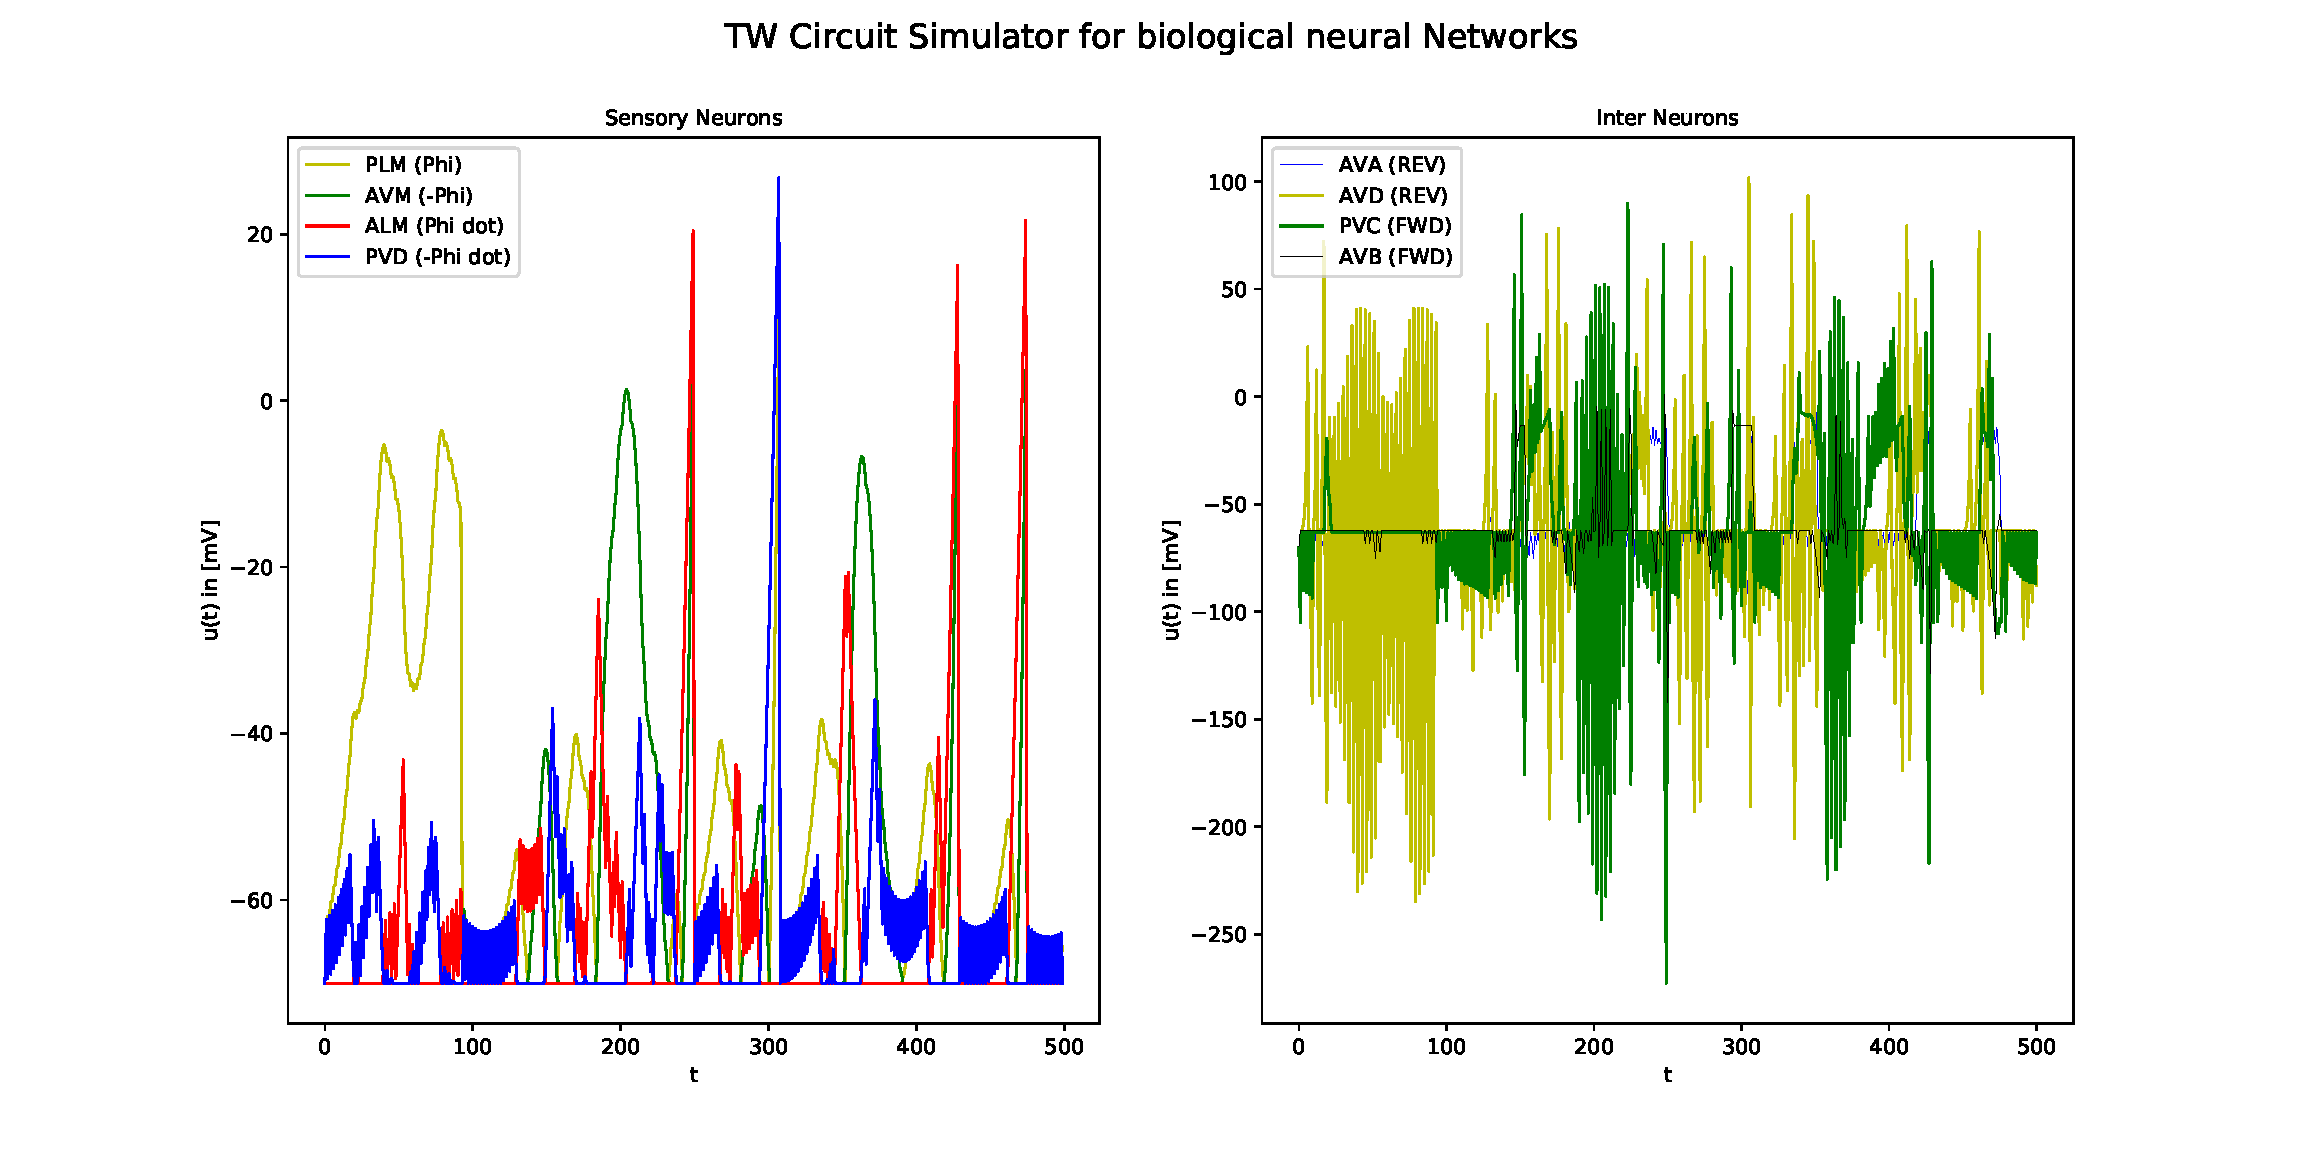
\includegraphics[width=16cm]{figures/chap_implement/plot_membranpot.pdf}
		\caption{Plot der Membranpotentiale von Inter- und Sensorneuronen}
		\label{fig:plot_membr}
	\end{figure}
	Weiterhin wird standardmäßig neben den Membranpotentialen auch der anliegende Synapsenstrom an jeder Nervenzelle geplottet. Diese Veranschaulichung gibt Aufschluss über die gewählten Parameter und das Feuerverhalten im internen neuronalen Netzwerk.
	\begin{figure}[H] %[!t] ...
		\centering
		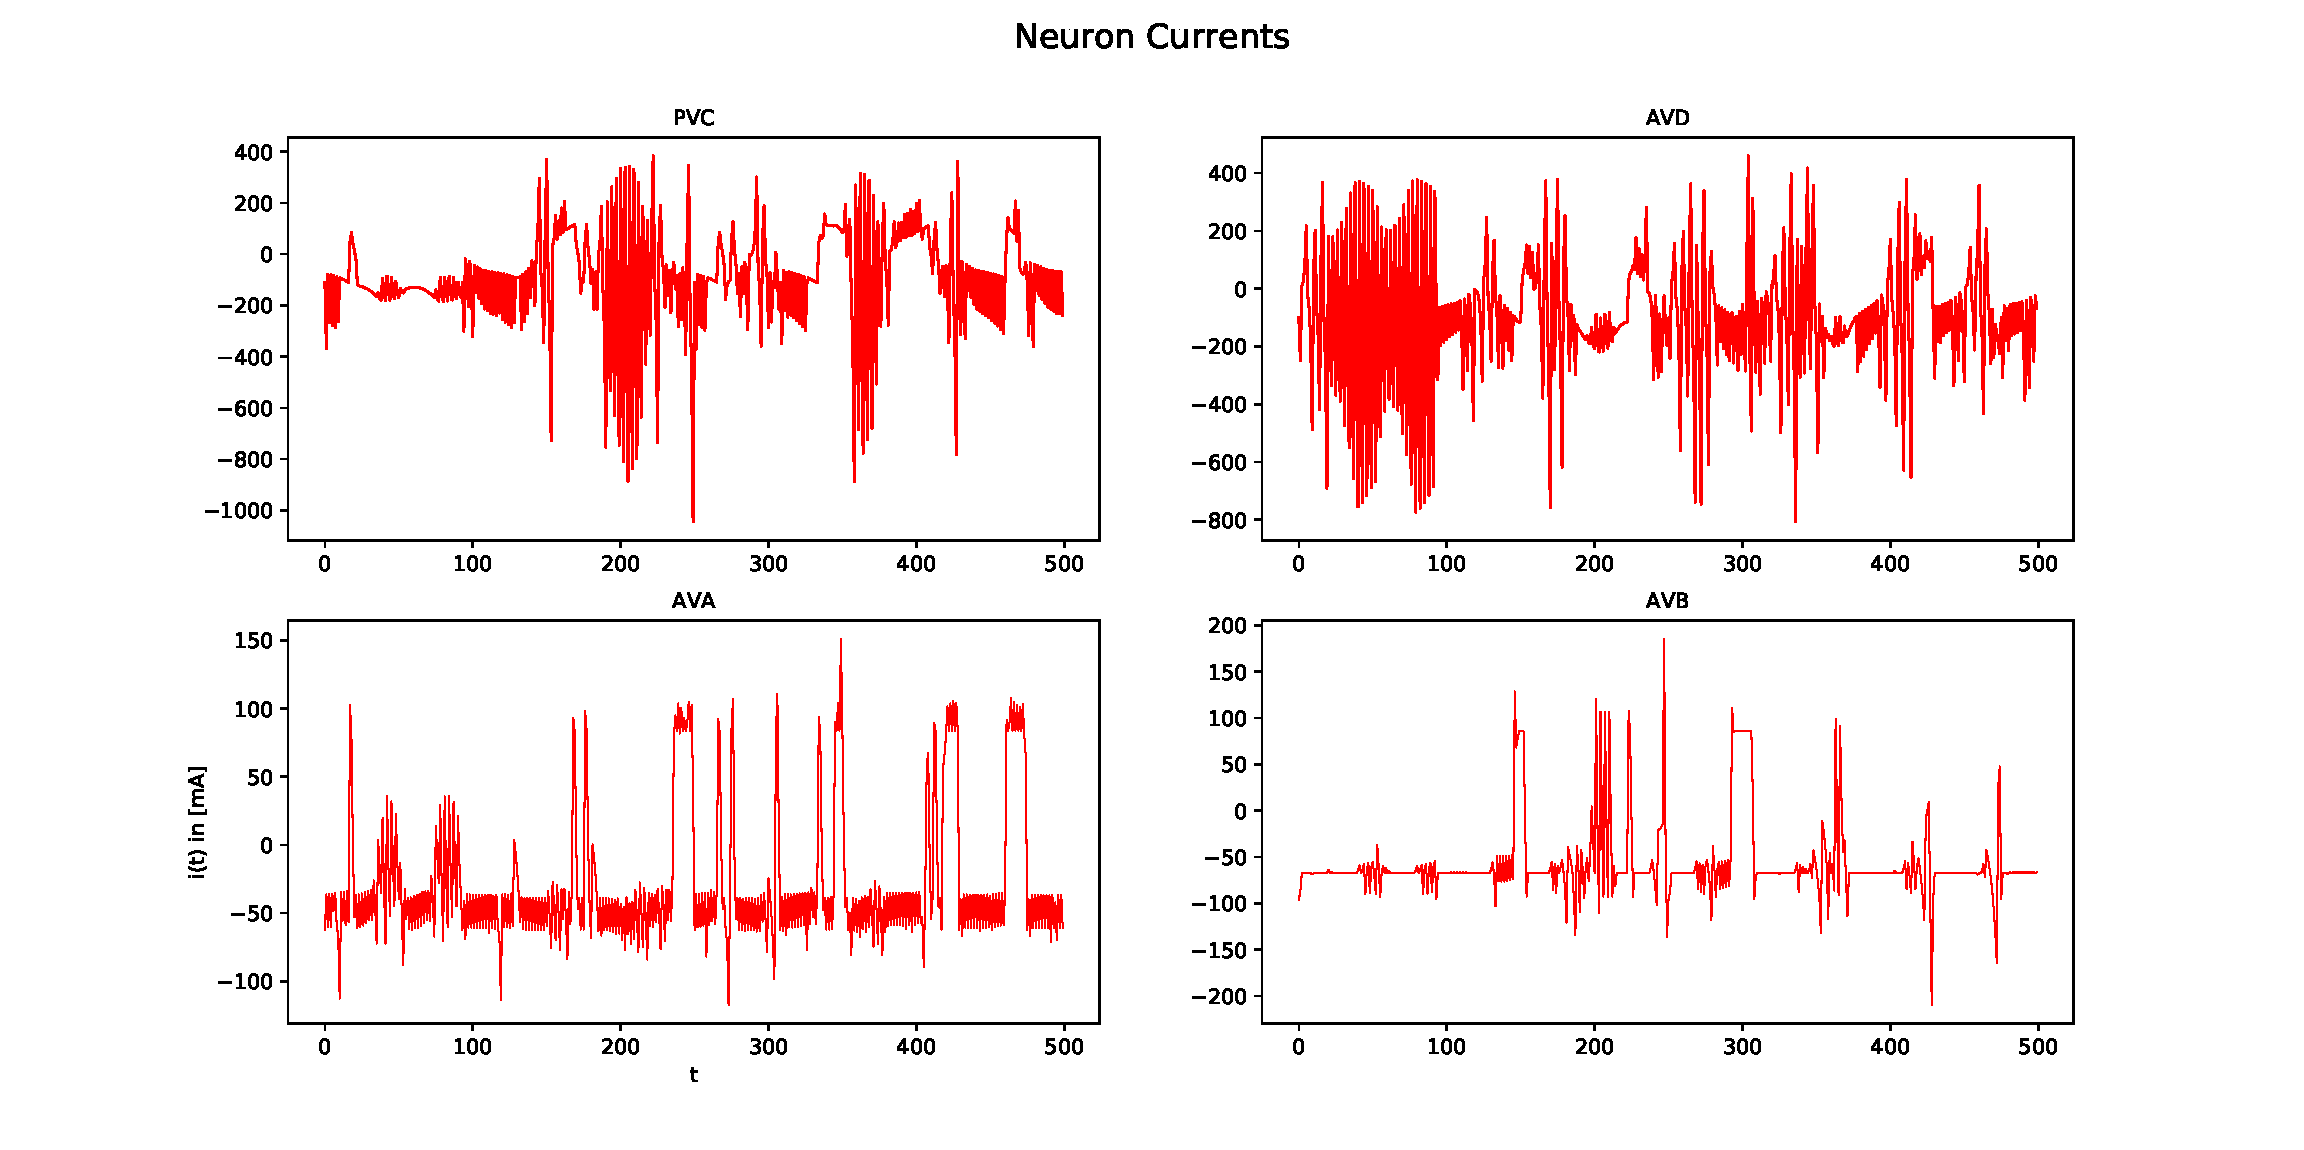
\includegraphics[width=16cm]{figures/chap_implement/plot_synstrom.pdf}
		\caption{Plot der anliegenden Ströme aus Stimulus, Synapsen und Gap-Junctions}
		\label{fig:plot_synstrom}
	\end{figure}

% ***
\section{Sonstige Implementierung}
\label{sec:imp_sonst}
% ***
	Neben den prominenten Modulen wurden im Laufe der Zeit mehrere hilfreiche Nebenmodule und Funktionen implementiert sowie notwendige Pakete genutzt.
	\subsection{Zentraler Ort für Parameter}
		Um einen zentralen Ort für verschiedene Größen und Parameter zu schaffen, wurde das Modul \texttt{parameters.py} erstellt. Dieses Modul wird im gesamten Programm eingebunden und dient als globale Informationsbasis. Nur wenige Größen können verändert werden wie bspw. die Transitionsmatrizen des neuronalen Netzes oder manche Parameter zur Berechnung von Synapsenströmen und Membranpotentialen. Alle weiteren Daten werden automatisch berechnet und im Laufe der Simulation bereitgestellt.
	\subsection{Speicherung von Daten}
		Ein Problem, welches über die Implementierung aufkam, war die Speicherung von Dateien in s.g. Dump-Files. Nach einer erfolgreichen Simulation von Parametern soll der beste Parametersatz zur weiteren Analyse gespeichert werden. Dazu liefert Python die Bibliothek \texttt{Pickle}, welche verschiedene Datentypen seriell in ein kompaktes Binärformat konvertiert und in der \texttt{.p} Dateiendung speichert. Dieser Vorgang ist jedoch besonders mit Python 2.7 verhältnismäßig langsam und beeinträchtigt die Performance der Simulation. Darüber hinaus besteht eine Inkompatibilität des Dateiformats zum einen zwischen verschiedenen Python-Versionen, zum anderen unter unterschiedlichen Betriebssystemen.\\
		Eine elegantere Möglichkeit bietet die Open Source Bibliothek \texttt{hickle}. Sie wird ähnlich wie \texttt{pickle} importiert und speichert die gewählten Parameter in einer \texttt{.hkl}-Datei. Die Daten werden anders als bei Pickle im s.g. HDF5 (Hierarchical Data Format 5) \cite{hdf5} gespeichert. Dies ist zum einen performanter, sorgt zum anderen für eine erheblich größere Kompatibilität unter Python-Versionen und Betriebssystemen.
	\subsection{Dateiinspektion}
		Besonders nach den ersten Simulationen ist die Inspektion der errechneten Parameter und Gewichte von äußerster Wichtigkeit. Hohe Rewards bedeuten nicht direkt, dass das neuronale Netz in jeder Situation richtig oder gut performt. Beispielsweise kann ein sehr guter Reward in der Bewegung des Pendels in Vorwärtsrichtung erreicht werden, obwohl die Parameter der Rückwärtsbewegung nicht sehr gut ausgereift sind. Daher wird ein Modul zur detaillierten Inspizierung der Dump-Dateien \texttt{inspect.py} geschrieben. Bei Aufruf einer Funktion dieses Moduls muss jeweils der Pfad der Dump-Datei übergeben werden. Die Datei wird geöffnet und die Parameter den entsprechenden Größen zugewiesen. Danach kann ein Konsolen-Output erfolgen oder ein Plot der gespeicherten Daten erzeugt werden.


%%% Local Variables: 
%%% mode: latex
%%% TeX-master: "main"
%%% End: 
